%IntroductionAndMotivation

%Add Oktoberfest-Situation-Picture and main station situation sketch in this section (the main station sketch also in the model/implementation section)

\subsection{Motivation}
As many commuters too, we all got annoyed by people rushing through the small corridor left in the Zurich main station hall (the path between burger king and groups meeting point) during the Oktoberfest, market days, concerts and other occasions when going from the platform, passing the meeting points in direction towards the Central and further on. So when thinking about a simulation project, this quickly crossed our minds.\\
In comparison to other pedestrian simulations, our simulation is special in different ways: this situation of a narrow but long corridor implies that there's not much space to avoid other pedestrians to the side, especially if there are lots of other people, whereas there is no need of path optimisation as the ultimate goal is to cross the hallway without crashing into someone else.\\
Being sometimes in such a situation inside that small corridor, we observed very special dynamics evolving between people rushing by, people just strolling around and people who want to talk to each other and so on.
%Add Oktoberfest-Situation-Picture here
%Maybe add sketch of situation here too?

\begin{figure}[h!]
	\centering
		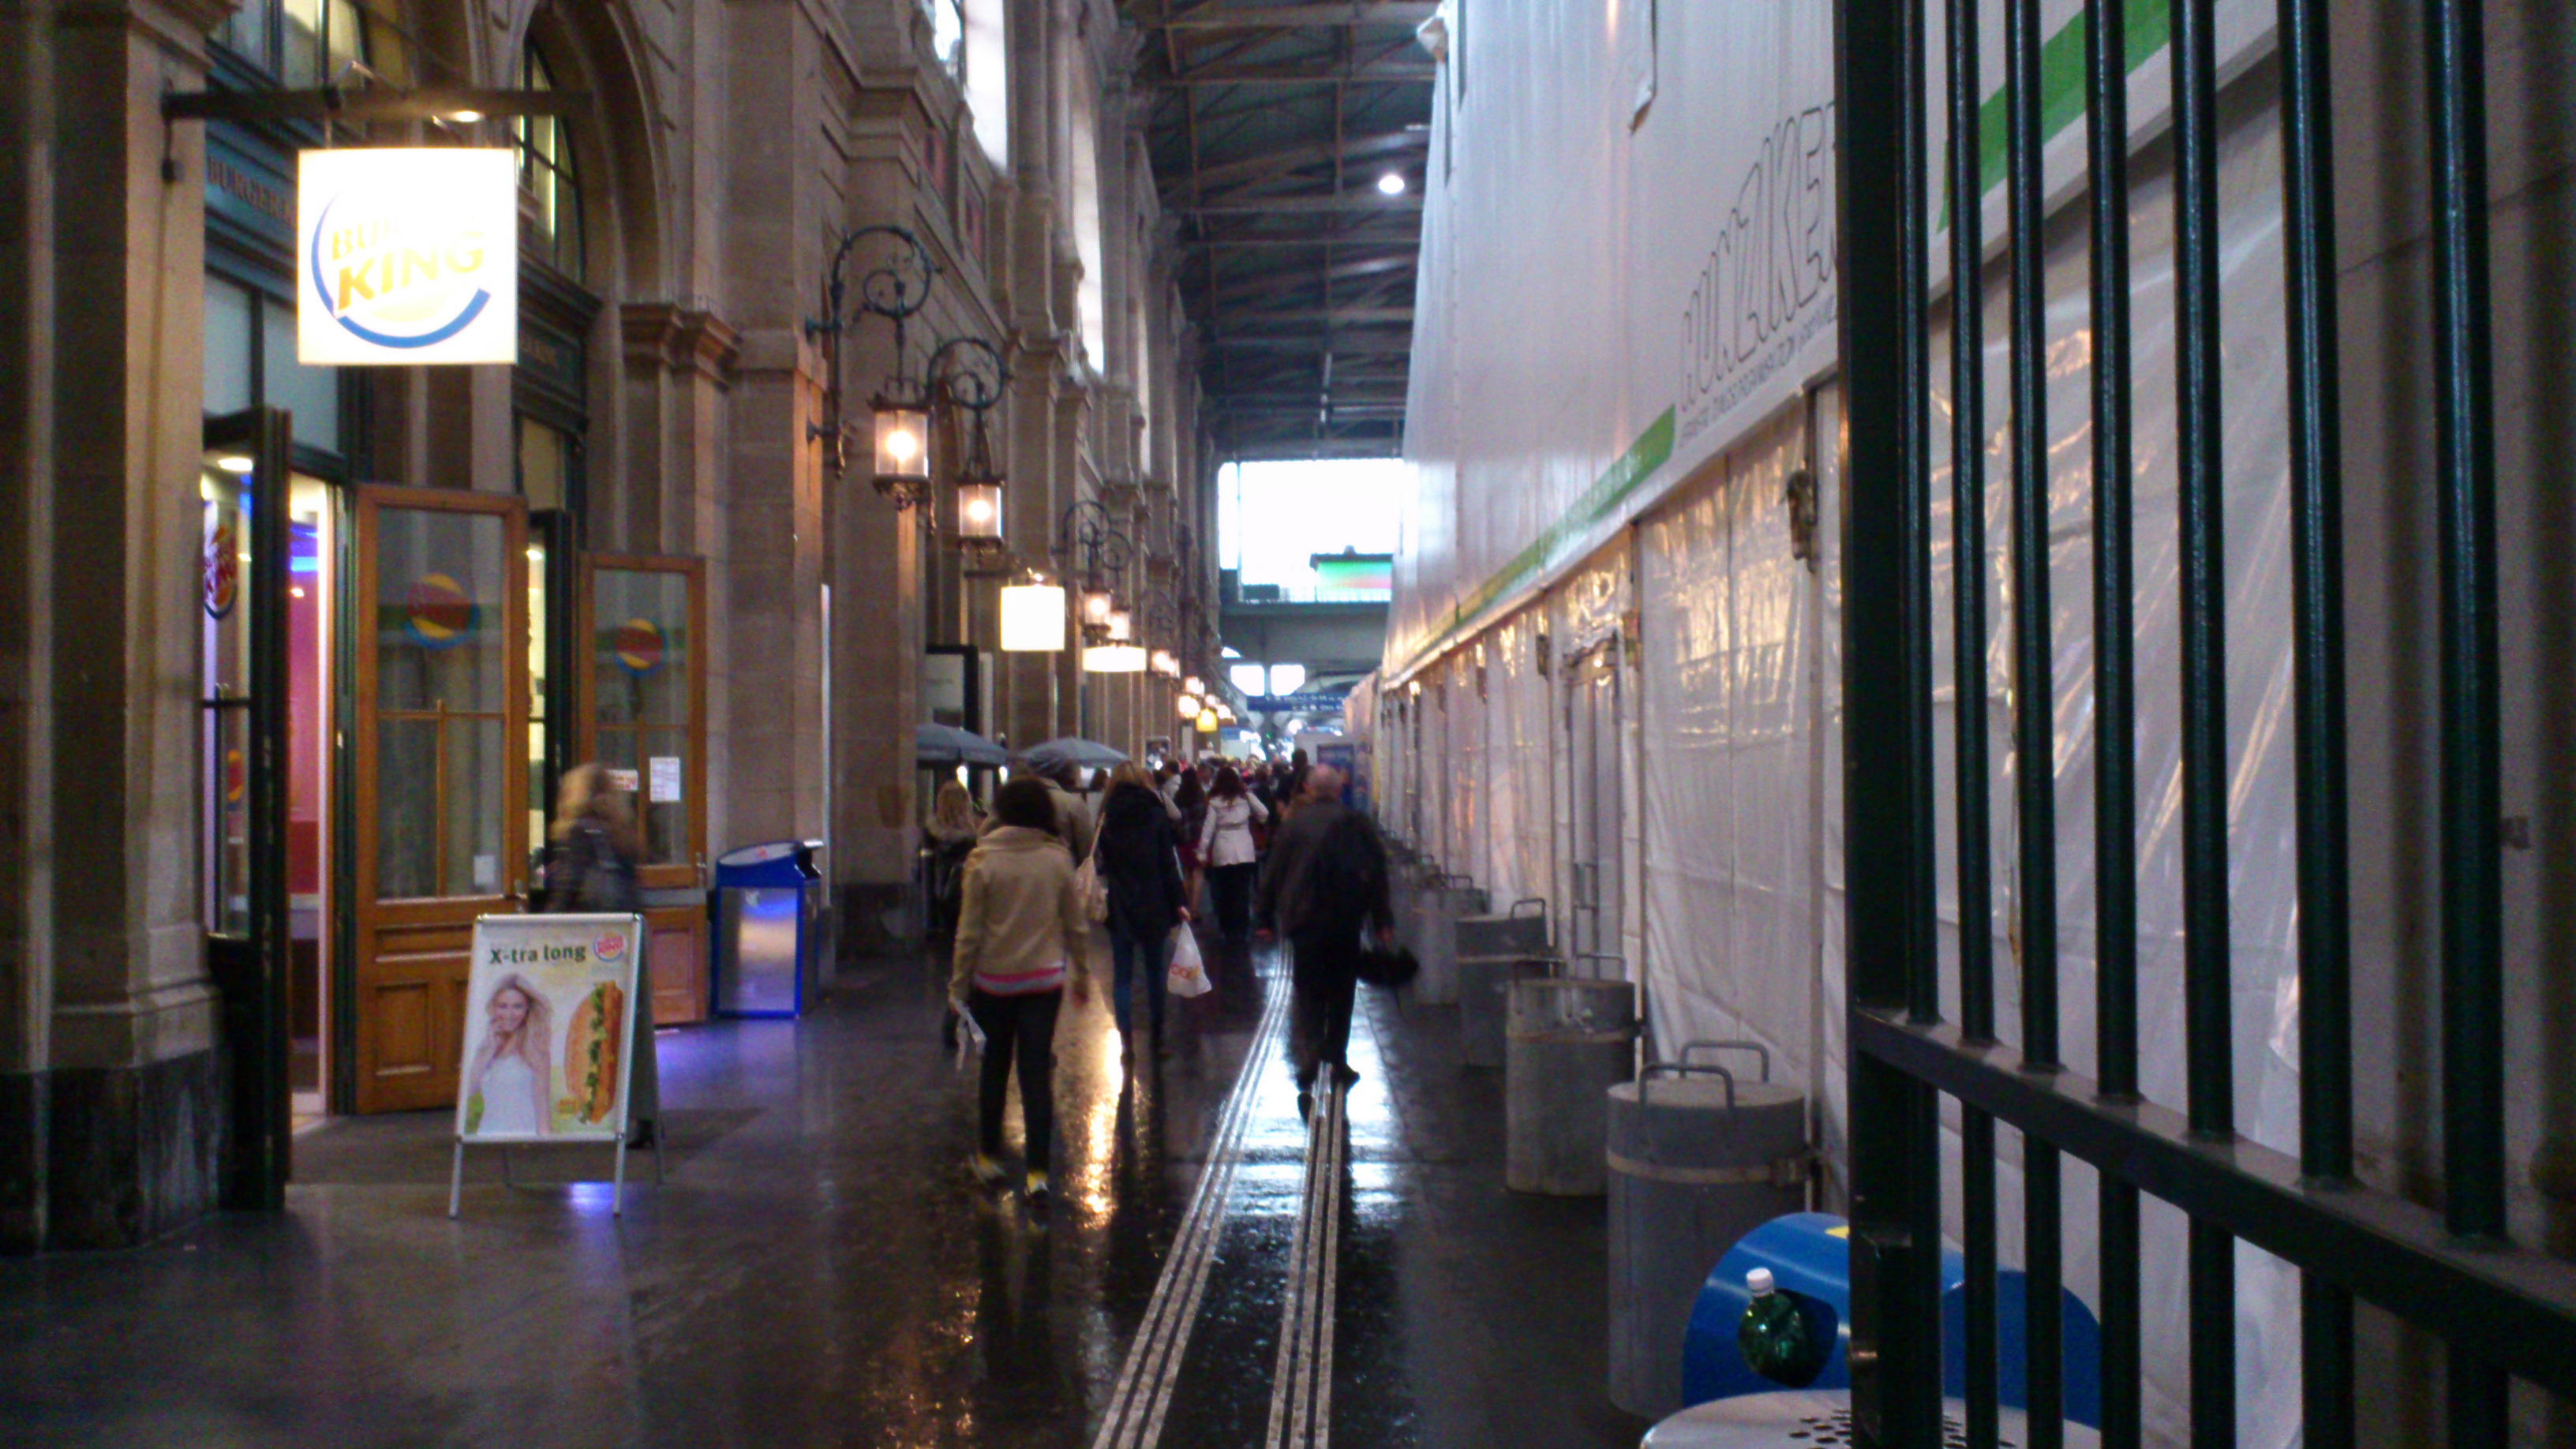
\includegraphics[width=0.90\textwidth]{pictures/oktoberfest2}
	\caption{Photo of the narrowed passage during the "Oktoberfest 2012".}
	\label{fig:oktoberfest2}
\end{figure}

\pagebreak

\subsection{Fundamental Questions}
The fundamental questions of our simulation project we started with were:
\begin{itemize}
\item We try to simulate the pedestrian flux of agents in a hallway in the following different situations: Rush hour (danger of jamming), much more agents in one direction than in the other, with an static obstacle (if possible), with aggressive/very fast or slow agents, random path agent (drunkard). Will the pedestrian flux run smoothly or will they block each other and be stuck?
\item Will the implementation of a rudimentary kind of thinking/looking ahead help to avoid blockages? If possible, we may determine the limits for which the goal of passing is achieved with and without this implementation and compare them.
\item Will there be group dynamics or similar behaviours of agents even if they're only programmed to walk to the other side, each on his own?
\end{itemize}

\noi As soon as the programming phase started, we realized there was a major point of importance about this work we all were aware of, but had forgot to think about beforehand. We did not want to start with a simulation already created, but build something "new" on our own. So we started off by creating our logic functions that would allow the agents to avoid crashing into other agents, then turned to the graphical part. As a consequence, new fundamental questions arose:
\begin{itemize}
\item Starting with the idea of looking ahead, how can we turn this into a rudimentary kind of intelligence?
\item How can we have a look at the main station situation but keep our agents as random as possible?
\item Using our own kind of rudimentary intelligence, will a form of collective behaviour follow? Will we be able to remodel the dynamics that appear when people start to rush forwards while other are considerable slower?
\end{itemize}

\subsection{Expected Results}
We thought that there would be lots of changes in the direction of walking to the left and right while trying to avoid other agents. With rising amount of agents we expected more jams, although this seems obvious. We thought that in our simulation we would have to deal with massive jams because the agents were not communicating with each other in any way. Our implementation of "looking ahead" as a form of intelligence would probably improve the people flux but only to a limited range. The formation of columns of people as a way to avoid the zig-zag-pattern of the agents' ways might appear.
